\documentclass[twoside]{article}
\usepackage{geometry}
\geometry{paperwidth=148mm,paperheight=210mm,margin=10mm}
\usepackage{graphicx}
\usepackage{stix}
\pagestyle{empty}\thispagestyle{empty}

\title{Compact notes on probability}
\author{Erik Ø. Sørensen}

% List of newcommands used in
% ``Notation in Econometrics:
% A Proposal for a Standard''
% by Karim Abadir and Jan Magnus
% Med et lite tillegg av Erik �. S�rensen: \defdas
%
\usepackage{amsfonts}
%\usepackage{amssymb}
\usepackage{graphics}
\usepackage{epsfig}
\usepackage{verbatim}

\usepackage{latexsym}
\usepackage{amsmath}
%%%
\newcommand{\newoperator}[3]{\newcommand*{#1}{\mathop{#2}#3}}
\newcommand{\renewoperator}[3]{\renewcommand*{#1}{\mathop{#2}#3}}
%
% Dette er min egen:
\newcommand{\defdas}{\mathrel{\raise0.095ex\hbox{$:$}\mkern-5mu = }}
%
% symbols C,N,Q,R,Z for sets
\newcommand{\SC}{\mathbb{C}}
\newcommand{\SN}{\mathbb{N}}
\newcommand{\SQ}{\mathbb{Q}}
\newcommand{\SR}{\mathbb{R}}
\newcommand{\SZ}{\mathbb{Z}}
%
% calligraphic capital letters
\newcommand{\calA}{\mathcal{A}}
\newcommand{\calB}{\mathcal{B}}
\newcommand{\calC}{\mathcal{C}}
\newcommand{\calD}{\mathcal{D}}
\newcommand{\calE}{\mathcal{E}}
\newcommand{\calF}{\mathcal{F}}
\newcommand{\calG}{\mathcal{G}}
\newcommand{\calH}{\mathcal{H}}
\newcommand{\calI}{\mathcal{I}}
\newcommand{\calJ}{\mathcal{J}}
\newcommand{\calK}{\mathcal{K}}
\newcommand{\calL}{\mathcal{L}}
\newcommand{\calM}{\mathcal{M}}
\newcommand{\calN}{\mathcal{N}}
\newcommand{\calO}{\mathcal{O}}
\newcommand{\calP}{\mathcal{P}}
\newcommand{\calQ}{\mathcal{Q}}
\newcommand{\calR}{\mathcal{R}}
\newcommand{\calS}{\mathcal{S}}
\newcommand{\calT}{\mathcal{T}}
\newcommand{\calU}{\mathcal{U}}
\newcommand{\calV}{\mathcal{V}}
\newcommand{\calW}{\mathcal{W}}
\newcommand{\calX}{\mathcal{X}}
\newcommand{\calY}{\mathcal{Y}}
\newcommand{\calZ}{\mathcal{Z}}
%
% bold lowercase and capital letters for vectors (v) and matrices (m)
\newcommand{\mA}{\bm A}
\newcommand{\va}{\bm a}
\newcommand{\mB}{\bm B}
\newcommand{\vb}{\bm b}
\newcommand{\mC}{\bm C}
\newcommand{\vc}{\bm c}
\newcommand{\mD}{\bm D}
\newcommand{\vd}{\bm d}
\newcommand{\mE}{\bm E}
\newcommand{\ve}{\bm e}
\newcommand{\mF}{\bm F}
\newcommand{\vf}{\bm f}
\newcommand{\mG}{\bm G}
\newcommand{\vg}{\bm g}
\newcommand{\mH}{\bm H}
\newcommand{\vh}{\bm h}
\newcommand{\mI}{\bm I}
\newcommand{\vi}{\bm i}
\newcommand{\mJ}{\bm J}
\newcommand{\vj}{\bm j}
\newcommand{\mK}{\bm K}
\newcommand{\vk}{\bm k}
\newcommand{\mL}{\bm L}
\newcommand{\vl}{\bm l}
\newcommand{\mM}{\bm M}
\newcommand{\vm}{\bm m}
\newcommand{\mN}{\bm N}
\newcommand{\vn}{\bm n}
\newcommand{\mO}{\bm O}
\newcommand{\vo}{\bm o}
\newcommand{\mP}{\bm P}
\newcommand{\vp}{\bm p}
\newcommand{\mQ}{\bm Q}
\newcommand{\vq}{\bm q}
\newcommand{\mR}{\bm R}
\newcommand{\vr}{\bm r}
\newcommand{\mS}{\bm S}
\newcommand{\vs}{\bm s}
\newcommand{\mT}{\bm T}
\newcommand{\vt}{\bm t}
\newcommand{\mU}{\bm U}
\newcommand{\vu}{\bm u}
\newcommand{\mV}{\bm V}
\newcommand{\vv}{\bm v}
\newcommand{\mW}{\bm W}
\newcommand{\vw}{\bm w}
\newcommand{\mX}{\bm X}
\newcommand{\vx}{\bm x}
\newcommand{\mY}{\bm Y}
\newcommand{\vy}{\bm y}
\newcommand{\mZ}{\bm Z}
\newcommand{\vz}{\bm z}
%
% bold Greek lowercase letters for vectors (v)
\newcommand{\valpha}{\bm \alpha}
\newcommand{\vbeta}{\bm \beta}
\newcommand{\vgamma}{\bm \gamma}
\newcommand{\vdelta}{\bm \delta}
\newcommand{\vepsi}{\bm \epsi}
\newcommand{\vvarepsilon}{\bm \varepsilon}
\newcommand{\vzeta}{\bm \zeta}
\newcommand{\veta}{\bm \eta}
\newcommand{\vtheta}{\bm \theta}
\newcommand{\viota}{\bm \iota}
\newcommand{\vkappa}{\bm \kappa}
\newcommand{\vlambda}{\bm \lambda}
\newcommand{\vmu}{\bm \mu}
\newcommand{\vnu}{\bm \nu}
\newcommand{\vxi}{\bm \xi}
\newcommand{\vpi}{\bm \pi}
\newcommand{\vrho}{\bm \rho}
\newcommand{\vsigma}{\bm \sigma}
\newcommand{\vtau}{\bm \tau}
\newcommand{\vupsilon}{\bm \upsilon}
\newcommand{\vphi}{\bm \phi}
\newcommand{\vchi}{\bm \chi}
\newcommand{\vpsi}{\bm \psi}
\newcommand{\vomega}{\bm \omega}
%
% bold Greek capital letters for matrices (m)
\newcommand{\mGamma}{\bm \varGamma}
\newcommand{\mDelta}{\bm \varDelta}
\newcommand{\mTheta}{\bm \varTheta}
\newcommand{\mLambda}{\bm \varLambda}
\newcommand{\mXi}{\bm \varXi}
\newcommand{\mPi}{\bm \varPi}
\newcommand{\mSigma}{\bm \varSigma}
\newcommand{\mUpsilon}{\bm \varUpsilon}
\newcommand{\mPhi}{\bm \varPhi}
\newcommand{\mPsi}{\bm \varPsi}
\newcommand{\mOmega}{\bm \varOmega}
%
% roman letters in mathematics
\newcommand{\rB}{\ensuremath{\mathrm{B}}}
\newcommand{\rC}{\ensuremath{\mathrm{C}}}
\newcommand{\rD}{\ensuremath{\mathrm{D}}}
\newcommand{\rF}{\ensuremath{\mathrm{F}}}
\newcommand{\rH}{\ensuremath{\mathrm{H}}}
\newcommand{\rL}{\ensuremath{\mathrm{L}}}
\newcommand{\rN}{\ensuremath{\mathrm{N}}}
\newcommand{\rt}{\ensuremath{\mathrm{t}}}
\newcommand{\rU}{\ensuremath{\mathrm{U}}}
%
\newcommand{\bin}{\ensuremath{\mathrm{bin}}}
\newcommand{\eu}{\ensuremath{\mathrm{e}}}
\newcommand{\iu}{\ensuremath{\mathrm{i}}}
\newcommand{\LN}{\ensuremath{\mathrm{LN}}}
\newcommand{\Po}{\ensuremath{\mathrm{Po}}}
%
\newcommand{\ped}[1]{\ensuremath{_\mathrm{#1}}} %pedex
\newcommand{\ap}[1]{\ensuremath{^\mathrm{#1}}} %apex
\renewoperator{\Re}{\mathrm{Re}}{\nolimits}
\renewoperator{\Im}{\mathrm{Im}}{\nolimits}
%
% letters for (partial) differentiation
%\newcommand{\rd}{\ensuremath{\mathrm{d}}}
\makeatletter
\newcommand{\rd}{\@ifnextchar^{\DIfF}{\DIfF^{}}}
\def\DIfF^#1{%
   \mathop{\mathrm{\mathstrut d}}%
   \nolimits^{#1}\gobblespace}
\def\gobblespace{\futurelet\diffarg\opspace}
\def\opspace{%
   \let\DiffSpace\!%
   \ifx\diffarg(%
   \let\DiffSpace\relax
   \else
   \ifx\diffarg[%
   \let\DiffSpace\relax
   \else
   \ifx\diffarg\{%
   \let\DiffSpace\relax
   \fi\fi\fi\DiffSpace}
\newcommand{\deriv}[3][]{\frac{\rd^{#1}#2}{\rd #3^{#1}}}
\newcommand{\pderiv}[3][]{\frac{\partial^{#1}#2}{\partial #3^{#1}}}
%
% operatornames
\newcommand{\bias}{\operatorname{bias}}
\newcommand{\col}{\operatorname{col}}
\newcommand{\corr}{\operatorname{corr}}
\newcommand{\cov}{\operatorname{cov}}
\newcommand{\dg}{\operatorname{dg}}
\newcommand{\diag}{\operatorname{diag}}
\newcommand{\E}{\operatorname{E}}
\newcommand{\etr}{\operatorname{etr}}
\newoperator{\ip}{\mathrm{int}}{\nolimits}
\newcommand{\kur}{\operatorname{kur}}
\newcommand{\median}{\operatorname{med}}
\newcommand{\MSE}{\operatorname{MSE}}
\newcommand{\plim}{\operatorname{plim}}
\newcommand{\rk}{\operatorname{rk}}
\newcommand{\sgn}{\operatorname{sgn}}
\newcommand{\tr}{\operatorname{tr}}
\newcommand{\var}{\operatorname{var}}
\renewcommand{\vec}{\operatorname{vec}}
\newcommand{\vech}{\operatorname{vech}}
%
% other definitions
\newcommand{\distr}{\sim}
\newcommand{\adistr}{\stackrel{a}{\distr}}
\newcommand{\diff}{\bigtriangledown}
\newcommand{\fordiff}{\bigtriangleup}
\newcommand{\mply}{\cdot}
\newcommand{\widebar}{\overline}
%
%\mathchardef\varepsilon="010F
%\mathchardef\epsilon="0122
%\mathchardef\eps="010F
\newcommand{\eps}{\epsilon}
\newcommand{\epsi}{\varepsilon}
%
\newcommand{\longto}{\longrightarrow}
\newcommand{\pto}{\stackrel{p}{\longrightarrow}}
\newcommand{\dto}{\stackrel{d}{\longrightarrow}}
\newcommand{\wto}{\stackrel{w}{\longrightarrow}}
%
\newcommand{\vvarsigma}{\bm \varsigma}
\newcommand{\score}{\vvarsigma}
\newcommand{\Infmat}{\bm\calI}
\newcommand{\Hesmat}{\bm\calH}
%
\newcommand{\vones}{\bm\imath}
\newcommand{\vzeros}{\boldsymbol{0}}
\newcommand{\mzeros}{\mathbf{O}}
%
\newcommand{\bcdot}{\raisebox{1pt}{\textbf{\large .}}}
\newcommand{\interior}[1]{\overset{\circ}{#1}}
%
\newcommand{\hspacesymbols}%
   {$\{x: x \in S, x$ satisfies $P\}\;\;$} %symbols index
\newcommand{\type}[1]{{\tt$\backslash$#1}}

\usepackage{bm}

%\theoremstyle{theorem}
\newtheorem{theorem}{Theorem}%[section]
\begin{document}
\maketitle
\sloppy
\frenchspacing

\noindent This set of compact notes is written to support the fall method camp
in probability and statistics for new Ph.D students at NHH Norwegian
School of Economics and is in no way intended to replace a proper
book on the topics. 

\tableofcontents

\newpage
\section{Probability}
Let us define a \textbf{sample space} of all possible outcome of some
event (a set). Example, role of a die: $\calS =\{1,2,3,4,5,6\}$. 
An \textbf{event} is a subset of $\calS$. Events are what we assign probability
to.

The set of possible events must be restricted to a $\mathbf{\sigma}$\textbf{-algebra} $\calA$,
a class of subsets of $\calS$ such that if $A\in\calS$ then $A^c\in\calA$, if $A_1,A_2,\dots\in \calF$,
then $\cup_{i=1}^\infty A_i \in \calA$. 

$P$ is a \textbf{probability set function} if $P(A)\geq0$ for all $A\in\calA$; $P(\emptyset)=0$; $P(\calS)=1$,
and if $A_1,A_2,\dots$ is a series of \textbf{disjoint} sets ($A_i\cap A_j\emptyset$ when $i\neq j$), then
$P(\cup_{i=1}^\infty A_i)=\sum_{i=1}^\infty P(A_i)$.


The triple $(\calS,\calA,P)$ is called a \textbf{probability space}.

For $A$ and $B$ in $\calA$, we define the \textbf{conditional probability} of $A$ given $B$
as \[ P(A|B) = P(A\cap B)/P(B),\] when $P(B)>0$. From the definition, we can find 
\textbf{Bayes rule}
as 
\[ P(B|A) = \frac{ P(A|B)\cdot P(B)}{P(A)}.\]

If $A$ and $B$ are events with positive probability, $A$ and $B$ are \textbf{independent} if
$P(A\cap B) = P(A)\cdot P(B)$, $P(A|B)=P(A)$, and $P(B|A)=P(B)$ (all equivalent). Independence
is symmetric but not transitive.

\section{Random variables}

A \textbf{random variable}  (r.v.) is a function from a sample space to the real numbers,
$X\!\!: \calS \rightarrow \SR$. The probability space on $\calS$ maps to a new
probability space on $\SR$ (there are regularity conditions). 



\subsection{Distribution}
A random variable $X$ is said to have a \textbf{distribution function} (d.f.) $F_X$
such that \[ F_X(s) = P( X\in (-\infty, s]).\] When the derivative of the
distribution function exists, it is called the \textbf{density} of $X$, and
$f_X(s)=F'_X(s)$. We then say $X$ is distributed \textbf{continuously}. General
properties: $f_X(s)\geq0$, $\int_a^b f_X(s)\rd s = P(X\in[a,b])$, and
$\int_{-\infty}^\infty f_X(s) \rd s = 1$. When clear from context, we drop the
subscripts (and sometimes also the limits of integration): $\int\! f(s)\rd s=1$.

For \textbf{discrete} r.v., we define the \textbf{probability mass function} (pmf) as
$p_X(s) = P(X\in\{s\})$ for $s\in\calS$. This is analogous to the density function.

\subsection{Expectation of a random variable}
Let $X$ be a random variable. If $X$ is a continuous r.v.
with pdf $f(x)$ and 
\(\int_{-\infty}^\infty |x|f(x) \rd x < \infty,\)
the \textbf{expectation} of $X$ exists as  
\[\E[X] = \int_{-\infty}^\infty xf(x) \rd x.\]
If $Y$ is a discrete random variable with pmf $p_Y$, 
$\E[Y]=\sum_y yp_Y(y)$.

Having different expressions for discrete and continuous random variables is awkward, since
sometimes we need to do theory for mixed variables or variables where we don't know the 
distribution. To find a more general way to express expectations, we need to extend
our notion of \emph{integration}, this is outside the scope of our method camp. But we sometimes
see expressions such at $\E[X]=\int\! x \rd F_X(x)$
or even $E[X]=\int_\Omega X(\omega) P(\rd \omega)$.

The k-th \textbf{moment} of $X$ is $\E [X^k]$ (when it exists).  We often write $\mu=\E[X]$ (the \textbf{mean}) and
$\sigma^2 = \E[(X-\mu)^2]$ (the \textbf{variance}). The k-th \textbf{central moment} 
is $\E [ (X-\mu)^k]$.

The function expectation $m_X(t)=\E[e^{tX}]$ is called the \textbf{moment generating function}
when it exists in an open ball around zero. When it exists, $m'(0)=\E[X]$, $m''(0)=\E[X^2]$ and
$m^k(0)=\E[X^k]$.

\subsection{Expectation results}
\begin{enumerate}
\item Let $X$ be a random variable and let $m$ be a positive integer. 
Suppos(e that $E[X^m]$ exists. If $k$ is an integer and $k < m$, then
$E[X^k]$ exists.
\item Let $u(X)$ be a nonnegative function of the random variable $X$. If
$E[u(X)]$ exists, then for every positive constant $c$,
$P(u(X)\geq c) \leq \frac{E[u(X)]}{c}$ (\textbf{Markov}).
\item Let the random variable $X$ have a distribution with
finite variance $\sigma^2$. Then for every $k>0$, 
$P(|X-\mu|\geq k\sigma) \leq \frac{1}{k^2}$ (\textbf{Chebyshev}).
\item If $\phi$ is convex on an open interval $I$ and $X$ is a random
variable whose support is contained in $I$ and has finite expectation,
then $ \phi(E[X]) \leq E[\phi(X)]$ (\textbf{Jensen}).




\end{enumerate}

\subsection{Functions of random variables}
If $X$ is a random variable and $g$ is a function, $Y=g(X)$ is another random variable.

In Figure~\ref{fig:frv}a, $Y=g(x)$ is an increasing function. 
Thinking about the distribution of $Y$, if we start from the primitives,
the distribution function for $Y$ is $F_Y(y) = P(Y\leq y)$. We can substitute
the definition of $Y$ into this: $F_Y(y) = P(g(X)\leq y)$, where this
substitution depends on $g$ being increasing. Continuing
the substitutions, $P(g(X) \leq y) = P( g^{-1}(g(X)) \leq g^{-1}(y)) = P(X\leq g^{-1}(y))$,
and we can conclude that $F_Y(y)= F_X(g^{-1}(y))$. The density follows by differentiation.

If instead $Y=h(X)$ and $h$ is decreasing (as in Figure ~\ref{fig:frv}b), we
start with a different inequality: If $h(X) \leq y$, then $X\geq h^{-1}(y)$,
and $F_Y(y) = P(X\geq h^{-1})) = 1 - P(X\leq h^{-1}(y)) = 1 - F_X(h^{-1}(y))$.

Either way, for increasing or decreasing $g$'s, taking derivatives we find that 
$f_Y(y) = f_X(g^{-1}(y)) \cdot | \rd g^{-1}(y)/\rd y|$.
The absolute value of the derivative controls for whether $g$ is increasing or decreasing.


\begin{figure}[tb]
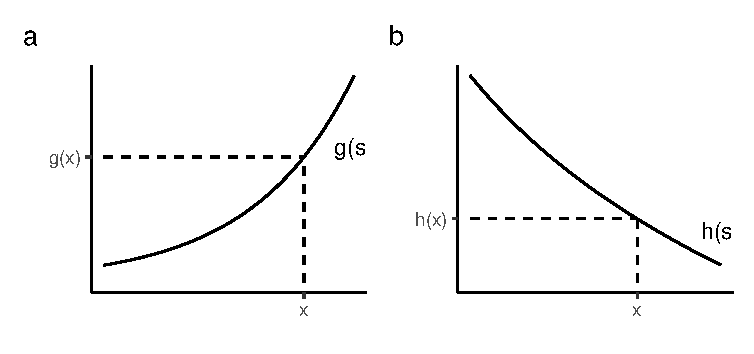
\includegraphics[width=0.95\textwidth]{../graphs/transformation_of_RV}

\caption{Functions of random variables}\label{fig:frv}
\end{figure}



\section{Random vectors}
Given a sample space $\mathcal{C}$. Consider the
two random variables $X_1$ and $X_2$, which assign to each element
$c$ of $\mathcal{C}$ an ordered pair of numbers
$X_1(c)=x_1$, $X_2(c)=x_2$. Then we say that $(X_1,X_2)$ is a
\textbf{random vector}. 

If $(X_1,X_2)$ has density $f_{X_1,X_2}(x_1,x_2)$, the \textbf{marginal density}
of $X_1$ is  $ f_{X_1}(x_1) = \int_{-\infty}^\infty f_{X_1,X_2}(x_1,x_2)\rd x_2$.

If $(X_1,X_2)$ has a density, the \textbf{conditional density} of $X_1$ given $X_2$ is
\[f_{X_1|X_2}(x_1|x_2)=\frac{f_{X_1,X_2}(x_1,x_2)}{f_{X_2}(x_2)},\]
for $f_{X_2}(x_2)>0$.

The \textbf{conditional expectation} is $\E[X_2|X_1=x_1] = \int_{-\infty}^\infty s
f_{X_2|X_1}(s|x_1) \rd s$.

Let $(X_1,X_2)$ have joint d.f. $F(x_1,x_2)$ and let $X_1$ and $X_2$ 
have marginal d.f.s $F_1(x_1)$
  and $F_2(x_2)$. Then $X_1$ and $X_2$ are \textbf{independent} if and only if 
$F(x_1,x_2)= F_1(x_1) F_2(x_2)$. 

If $X_1$ and $X_2$ are independent and $\E[u(X_1)]$ and $\E[v(X_2)]$ exist, then
$\E[u(X_1)v(X_2)] = \E[u(X_1)]\cdot \E[v(X_2)]$.


Let $(X_1,X_2)$ have joint CDF
  $F(x_1,x_2)$ and let $X_1$ and $X_2$ have marginal CDFs $F_1(x_1)$
  and $F_2(x_2)$. Then $X_1$ and $X_2$ are independent if and only if 
$$F(x_1,x_2)= F_1(x_1) F_2(x_2).$$


A vector $\mathbf{X}=(X_1,\dots,X_n)$ where each element is an \emph{independent} draw from the same distribution as the random variable
$X$ is known as a \textbf{random sample} of size $n$ of the variable
$X$.



\section{Estimation}


\section{Asymptotic theory}

\subsection{Convergence in probability}

$\{X_n\}$ is a sequence of random variables, and $X$ is a random variable, both
defined on the same sample space. Now $X_n$ \textbf{converges in probability} to $X$
if, for all $\epsilon>0$,
\[\lim_{n\rightarrow\infty} P( |X_n-X|\geq \epsilon) = 0.\] We say that
$\plim X_n = X$, or that $X_n \xrightarrow{P} X$.

\begin{theorem}
Let $\{X_n\}$ be sequence of iid random variables with common mean $\mu$ and
finite variance $\sigma^2$. If $\overline{X}_n = n^{-1}\sum_{i=1}^n X_i$, then
$\plim \overline{X}_n=\mu$. (Weak law of large numbers)
\end{theorem}

There are a number of results about how probability limits work:
\begin{enumerate}
\item Suppose $\plim X_n=X$ and $\plim Y_n=Y$. Then $\plim X_n+Y_n = X+Y$.
\item Suppose $\plim X_n=X$ and $a$ is a constant. Then $\plim a X_n = aX$.
\item Suppose $\plim X_n=a$ and the function $g$ is continuous at $a$. Then $\plim g(X_n)=g(a)$.
\item Suppose $\plim X_n=X$ and $\plim Y_n=Y$, then $\plim X_nY_n=XY$.
\end{enumerate}

The concept of probability limit is closely tied to the statistical concept
of consistency. Let $X$ be a r.v. with d.f. $F(s,\theta)$, for some $\theta\in\Omega$.
Let $X_1,X_2,\dots,X_n$ be a random sample on $X$, and let $T_n$ be a statistic.
$T_n$ is a \textbf{consistent} estimator of $\theta$ if $\plim T_n = \theta$.

\subsection{Convergence in distribution}
$\{X_n\}$ is a sequence of random variables and $X$ is a random variable,
let $F_{X_n}$ and $F_X$ be the respective distribution functions. Let 
$C(F_X)$ be the set of points at which $F_X$ is continuous. Now $X_n$ \textbf{converges in
distribution} to $X$ if $\lim_{n\rightarrow\infty} F_{X_n}(x) = F_X(x)$ for all
$x\in C(F_X)$, and we sometimes write \[X_n \xrightarrow{D} X.\]

Like for convergence in probability, we have some theorems about convergence in distribution:

\begin{enumerate}
\item If $X_n$ converges to $X$ in probability, then $X_n$ converges to $X$ in distribution.
\item If $X_n$ converges to the constant $b$ in distribution, then $X_n$
converges to $b$ in probability.
\item If $X_n$ converges to $X$ in distribution and $Y_n$ converges in probability to $0$,
then $X_n+Y_n$ converges to $X$ in distribution.
\item If $X_n$ converges to $X$ in distribution and $g$ is a continuous function on the support
of $X$, then $g(X_n)$ converges to $g(X)$ in distribution.
\item $X_n$, $X$, $A_n$, and $B_n$ are random variables and $a$ and $b$ are constants. 
If $X_n$ converges to $X$ in distribution, $\plim(A_n)=a$, and $\plim(B_n)=b$, then
\[ A_n + B_n X_n \xrightarrow{D} a + bX.\]
\end{enumerate}


\subsection{The Central Limit Theorem}
There is a whole literature about generalizing central limit theorems. A basic one:

\begin{theorem}
Let $X_1,X_2,\dots,X_n$ denote a random sample from a distribution with mean
$\mu$ and positive variance $\sigma^2$. Then the random variable \[ Y_n =
\left(\sum_{i=1}^n X_i - n\mu \right)/\sqrt{n}\sigma =
\sqrt{n}(\overline{X}_n-\mu)/\sigma\] converges in distribution to a random
variable with a normal distribution $N(0,1)$. 
\end{theorem}

A simple proof can be constructed for the subset of cases where $X$ has a moment generating
function, the trick is to do a second order Taylor-approximation of the moment generating
function of $X-\mu$. 

The $\mathbf{\Delta}$\textbf{-rule} is often useful in conjunction with the CLT.
It says that 

\begin{theorem}
If $\{X_n\}$ is a sequence of random variables such that $\sqrt{n}(\overline{X}_n-\theta)$
converges to $N(0,\sigma^2)$ in distribution, $g$ is a differentiable function at $\theta$,
and $g'(\theta)\neq 0$, then 
\[ \sqrt{n}\left(g(X_n) - g(\theta)\right) \xrightarrow{D} 
N\left(0, \left(g'(\theta)\right)^2\sigma^2\right).\]
\end{theorem}
This can be proven with a Taylor expansion. 

The $\Delta$-rule is the default approach to calculating the distribution of derived
statistics. If we can show that the CLT applies to some moments or parameters,
and we are interested in a function of these moments or parameters, we can use the 
$\Delta$-rule to calculate the distribution of these functions. Statistical packages
will often do this automatically (example: Stata's \texttt{testnl} command).

\section{Math facts}
In this section, there are some mathematical facts that turn out to be useful
for probability and statistics but isn't really part of statistics itself.

The \textbf{exponential function}, written $e^s$ or $\exp(s)$ is important. Can be defined by the
series expansion \[ e^x = \sum_{k=0}^\infty \frac{x^k}{k!},\] and $\exp'(s)=\exp(s)$.
It is also the case that \[ e^x = \lim_{n\rightarrow \infty} \left( 1 + \frac{x}{n} \right)^n. \]

If $\psi$ is some function such that $\psi(n) \rightarrow 0$ as $n\rightarrow\infty$,
then \[ \lim_{n\rightarrow\infty} \left(1 + \frac{x}{n} + \frac{\psi(n)}{n}  \right)^n = e^x,\]
since the $\psi(n)/n$ term vanishes faster than $x/n$.

A useful formulation of \textbf{Taylor's formula} is that for continuous and at
least twice differentiable functions functions $m\!\!\!:\!\!\SR \rightarrow \SR$, there
exists a number $\xi$ between $0$ and $t$ such that \[ m(t) = m(0) + m'(0) t +
\frac{1}{2} m''(\xi) t^2.\]


\end{document}